\section{Модификации и бутстреп-t интервал}

\footnote{Этот раздел содержит более сложный материал и может быть пропущен при первом прочтении.}С бутстреп-t процедурой нахождения доверительного интервала связаны как вычислительные проблемы, так и проблемы интерпретации. В знаменателе $Z^{*}(b)$ стоит $\widehat{\text{se}}^{*}(b)$, стандартное отклонение $\widehat{\theta}^{*}$ для бутстреп выборки $\textbf{x}^{*b}$. Для примера данных мыши, где  $\widehat{\theta}$ - среднее значение, мы использовали оценку методом подстановки:
\begin{gather}\label{12.23}
\widehat{\text{se}}^{*}(b) = \left\{\sum_{1}^{n} \frac{(x_{i}^{*b} -  \overline{x}^{*b})^{2}}{n^{2}}\right\}^{\frac{1}{2}},
\end{gather}
где $x_{1}^{*b}, x_{2}^{*b},\ldots,x_{n}^{*b}$ --- это бутстреп выборка.

Сложность возникает, когда $\widehat{\theta}$ более сложная статистика, для которой не существует простой формулы стандартной ошибки. Как мы видели в главе 5, формулы стандартной ошибки существуют для очень небольшого числа статистических данных, и поэтому нам потребуется вычислить начальную оценку стандартной ошибки \textit{для каждой начальной выборки}. Это подразумевает два вложенных уровня бутстреп выборки. Теперь для оценки стандартной ошибки может быть достаточно $B = 25$, в то время как для вычисления процентилей необходимо $B = 1000$. Следовательно, общее количество бутстреп равно 25 · 1000 = 25000, внушительное число, если $\widehat{\theta}$ сложно вычислима.

Вторая трудность с бутстреп-t интервалом заключается в том, что он может работать хаотично в непараметрической постановке с малой выборкой. Влияние этой неприятной особенности можно уменьшить. Рассмотрим, например, данные юридической школы из таблицы 3.1, для которой  $\widehat{\theta}$ - коэффициент корреляции выборки. При построении бутстреп-t интервала для $\widehat{\text{se}}^{*}(b)$ мы использовали оценку стандартной ошибки с B = 25 бутстреп выборками. Как упоминалось выше, общая процедура включает два вложенных уровня бутстреп выборок. Всего было сгенерировано 1000 значений  $\widehat{\theta}^{*}$, так что всего было использовано 25000 бутстреп выборок. Полученный ранее $90 \%$ бутстреп-t интервал был равен [-0.026, 0.90]. Для коэффициента корреляции хорошо известно (см. стр. 54), что если мы построим доверительный интервал для преобразованного параметра:
\begin{gather}\label{12.24}
\varphi = 0.5 \log(\frac{1+\theta}{1 - \theta}),
\end{gather}
затем преобразуем граничные точки с помощью обратного преобразования $(\exp(2\varphi) - 1)/(\exp(2\varphi) + 1)$, получаем улучшенный интервал. Если посчитать $90\%$ бутстреп-t доверительный интервал для $\varphi$ для данных о юридической школе, а затем преобразовать его обратно, мы получим интервал для $\theta$ [0.45, 0.93], который окажется намного короче, чем интервал, который был получен без преобразования. Если посмотреть на более высокий доверительный уровень, например $ 98\% $, границы будут равны [-0.66, 1.03] для интервала, посчитанного без преобразования, и [0.17, 0.95] для интервала посчитанного с использованием преобразованием. Обратите внимание, что первый интервал выходит за пределы допустимого диапазона для коэффициента корреляции! Таким образом, использование (не модифицированной) процедуры бутстреп-t для этой и других проблем может привести к интервалам, которые часто бывают слишком широкими и выходят за пределы допустимого диапазона для параметра. 

Другими словами, бутстреп-t интервал не является \textit{инвариантным относительно преобразований}. Важно, какая именно шкала используется для построения интервала, и одни шкалы подходят лучше других. В примере с коэффициентом корреляции преобразование (\ref{12.24}), является подходящим, если данные имеют двумерное нормальное распределение, и в целом хорошо подходит в этом случае. Однако для большинства случаев мы не знаем, какое именно преобразование применить, и это является главным каменем преткновения для построения бутстреп-t доверительного интервала.

Один из вариантов решения этой проблемы - использовать бутстреп для оценки соответствующего преобразования используя сами данные, а затем использовать это преобразование для построения бутстреп-t доверительного интервала. Посмотрим, как это можно сделать. Пусть $\theta$ коэффициент корреляции, положим $\widehat{\varphi} = 0.5 \log(\frac{1+\widehat{\theta}}{1 - \widehat{\theta}}),$ $\varphi = 0.5 \log(\frac{1+\theta}{1 - \theta})$. Получим:
\begin{gather}\label{12.25}
\hat{\varphi} - \varphi \  \dot{\sim} \  \mathrm{N}(0, \ \frac{1}{n - 3}).
\end{gather}
Это преобразование приближенно делает дисперсию устойчивой и нормализует оценку $\widehat{\theta}$. Было бы удобно иметь автоматический метод нахождения таких преобразований. Однако, обычно невозможно одновременно нормализовать оценку и обеспечить устойчивость дисперсии. Похоже, что для того чтобы использовать бутстреп-t доверительные интервалы важно второе свойство: метод лучше работает для параметров с устойчивой дисперсией. Пусть, $X$ - случайная величина со средним значением $\theta$ и стандартным отклонением $s(\theta)$, которое зависит от $\theta$, то аргумент ряда Тейлора (задача 12.4) показывает, что преобразование $g(x)$ с производной
\begin{gather}\label{12.26}
g'(x) = \frac{1}{s(\theta)},
\end{gather}
обладает тем свойством, что дисперсия $g(X)$ приблизительно константа. Эквивалентно 
\begin{gather}\label{12.27}
g(x) = \int_{}^x \frac{1}{s(u)}du.
\end{gather}
В данной задаче $X$ это $\widehat{\theta}$, и для каждого $u$ нам нужно знать $s (u)$, стандартную ошибку $\widehat{\theta}$, при условии что $\theta = u$, чтобы применить (\ref{12.27}).Будем писать $s(u) = \text{se}(\widehat{\theta}|\theta = u)$. Конечно, $\text{se}(\widehat{\theta}|\theta = u)$ обычно неизвестно, однако мы можем использовать бутстреп для его оценки. Затем мы вычисляем бутстреп-t интервал для параметра $\varphi = g(\theta)$ и преобразуем его используя обратную функцию $g^{-1}$, чтобы получить интервал для $\theta$. Подробности этого процесса показаны в алгоритме 12.1. Дополнительные подробности реализации можно найти в Tibshirani (1988).

\begin{algorithm}
\caption{Вычисление бутстреп - t интервала с устойчивой дисперсией}\label{12.1}
1. Сгенерируйте $B_{1}$ бутстреп выборок и для каждой выборки $x^{*b}$ вычислите бутстреп репликацю $\widehat{\theta}^{*}(b)$. Возьмите $B_{2}$ бутстреп выборок из $x^{*b}$ и оцените стандартную ошибку
$\widehat{\text{se}}(\widehat{\theta}^{*}(b))$.

2. Подстроить кривую под точки $[\widehat{\theta}^{*}(b), \widehat{\text{se}}(\widehat{\theta}^{*}(b))]$, чтобы получить гладкую оценку функции $\text{se}(\widehat{\theta}|\theta = u)$.

3. Оцените преобразование, стабилизирующее дисперсию $g(\widehat{\theta})$ по формуле (\ref{12.27}), используя численное интегрирование.

4. Используя новую $B_{3}$ бутстреп выбороку, вычислите бутстреп - t интервал для $\varphi = g(\theta)$. Поскольку стандартная ошибка $g(\widehat{\theta})$ примерно постоянна как функция от $\theta$, нам не нужно оценивать знаменатель в величине $(g(\widehat{\theta})^{*} - g(\widehat{\theta}) / \widehat{\text{se}})$ и можно установить его равным одному.

5. Отобразите граничные точки интервала обратно в ту же шкалу что и $\theta$ с помощью преобразования $g^{-1}$.
\end{algorithm}

На левом рисунке 12.2 показан пример для данных юридического факультета. Было сгенерировано $B_{1} = 100$ бутстреп выборок, и для каждой из них был вычислен коэффициент корреляции и бутстреп оценка его стандартной ошибки с использованием $B_{2} = 25$ бутстреп выборок второго уровня; таким образом, получается вложенный бутстреп, который содержит $100 \cdot 25 = 2500$ бутстреп выборок (эмпирические данные показывают, что 100 выборок первого уровня являются приемлимыми). Обратите внимание на сильную зависимость $\text{se}(\widehat{\theta}^{*})$ от ${\widehat{\theta}}^{*}$. Мы провели через этот график гладкую кривую, чтобы получить оценку $\text{se}(\widehat{\theta}|\theta = u)$, и применили формулу (\ref{12.27}), чтобы получить оценку преобразования $g(\widehat{\theta})$, обозначенную сплошной кривой на среднем рисунке. Пунктирная кривая на среднем рисунке это преобразование (\ref{12.24}). Кривые очень похожи, но разные; мы бы ожидали, что они совпадают, если бы выборка была проведена из двумерной нормальной генеральной совокупности. Правый рисунок такой же как левый, для $\widehat{\varphi}^{*} = g(\widehat{\theta}^{*})$ вместо $\widehat{\theta}^{*}$. Обратите внимание, как уменьшилась зависимость.

\begin{figure}[H]
\center{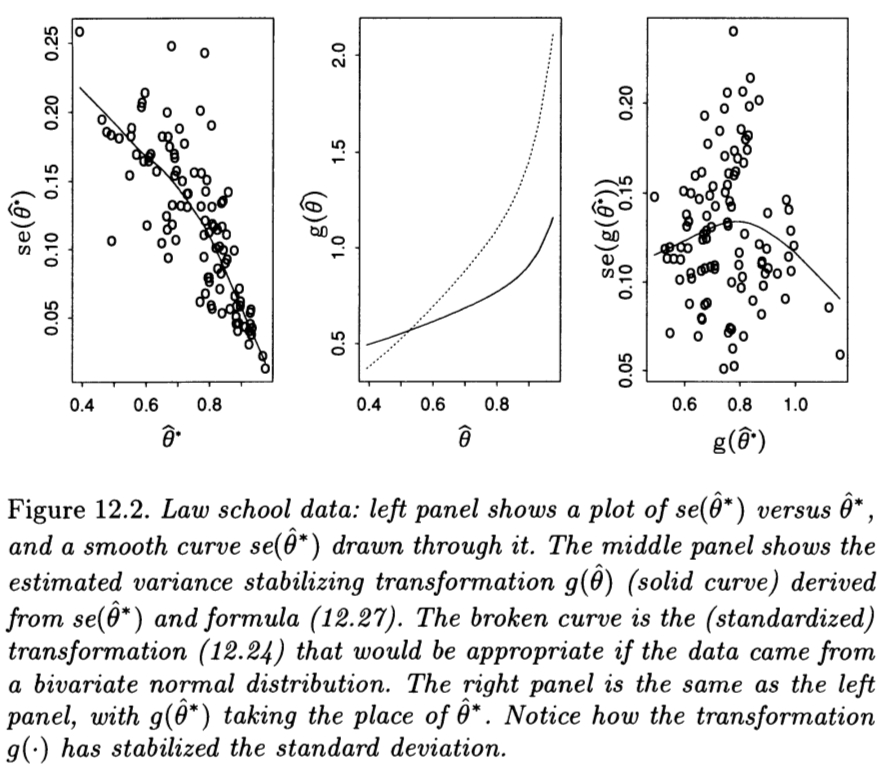
\includegraphics[width=1 \linewidth]{12.3.png}}
\end{figure}


Используя $ B_{3} = 1000$ бутстреп выборок, полученные $90\%$ и $98\%$ доверительные интервалы для коэффициента корреляции оказываются равными [0.33, 0.92] и [0.07, 0.95]. Оба интервала короче, чем полученные без преобразования, и лежат в пределах допустимых значений [-1, 1] для коэффициента корреляции. Общее количество бутстреп выборок равно 2500 + 1000 = 3500, что намного меньше чем 25 000 для обычной бутстреп-t процедуры.

Важным дополнительным свойством преобразования $\widehat{\varphi} = g (\widehat{\theta})$ является то, что оно позволяет нам игнорировать знаменатель t статистики  на 4 шаге. Это связано с тем, что стандартная ошибка приблизительно равна константе, и, следовательно, можно предположить, что она равна 1. Как следствие, как только преобразование $\widehat{\varphi} = g (\widehat{\theta})$ было получено, построение бутстреп-t интервала не требует вложенной выборки.

Другой подход к решению проблем с бутстреп-t интервалом совершенно иной. Вместо того, чтобы сосредотачиваться на статистике вида $Z = \frac{\widehat{\theta} - \theta}{\widehat{\text{se}}}$, мы работаем напрямую с бутстреп распределением $\widehat{\theta}$, получая инвариантность преобразования.
Этот подход описывается в следующих двух главах, а кульминацией является процедура «BCa» из главы 14. Как и бутстреп-t метод, «BCa» дает более точные интервалы, чем стандартные нормальные или t интервалы.

Функция языка S для вычисления бутстреп-t доверительных интервалов описана в Приложении. Он включает опцию автоматической стабилизации дисперсии.
